\documentclass[../main]{subfiles}

\begin{document}
\section{Numerical experiments} \label{sec:pgm:experiments}
In this section, we present some numerical results using \cref{alg:pgm_MO} for the problems in \cref{sec:pgm:robust}. The experiments are carried out on a machine with a 1.8GHz Intel Core i5 CPU and 8GB memory, and we implement all codes in MATLAB R2017a. We consider the problem \cref{eq:MOO}, where $n = 5,\, m = 2,\, f_i(x) = \frac{1}{2} x^\T A_i x + a_i^\T x,\, g_i(x) = \max_{u \in {\mathcal{U}}_i } \hat{g}_i (x,u),\ A_i \in \setR^{n \times n},\, a_i \in \setR^n$, and $\hat{g}_i\colon \setR^n \to \setR,\, i = 1,\ldots, m$. Here, we assume that each $A_i$ is positive semidefinite, so it can be decomposed as $A_i = M_i M_i^\T$, where $M_i \in \setR^{n \times n}$. We generate $M_i$ and $a_i$ by choosing every component randomly from the standard normal distribution. To implement \cref{alg:pgm_MO}, we make the following choices.
\begin{remark}
\begin{itemize}
\item Every component of $x^0$ is chosen randomly from the standard normal distribution.
\item In Experiments 1 and 3, we set the constant $\ell = 5$. In Experiment 2, we set the constant $\ell = 7$.
\item The terminate criteria is replaced by $\|d^k\| < \varepsilon \coloneqq 10^{-6}$.
\end{itemize}
\end{remark}

Also, we run each one of the following experiments 100 times from different initial points, and with $\delta = 0, 0.05, 0.1$. Naturally, when $\delta = 0$, no uncertainties are considered.
\subsection*{Experiment 1}
In the first experiment, we solve the problem of \cref{sec:pgm:robust:QP}. We assume that $g_i(x) = \max_{u \in \mathcal{U}_i } u^\T x,\, i = 1,2$, where $\mathcal{U}_1 = \{u \in \setR^5\mid -\delta \leq u_i \leq \delta,\, i = 1,\dots,5 \}$ and $\mathcal{U}_2 = \{u \in \setR^5\mid -\delta \leq (Bu)_i \leq \delta,\, i = 1,\dots,5 \}$. Here, every component of $B \in \setR^{5 \times 5}$ is chosen randomly from the standard normal distribution and $\delta \geq 0$. We use the MATLAB solver \emph{linprog} to solve \cref{eq:lp} and \emph{quadprog} to solve \cref{eq:qp}. \cref{fig:experiment1} is the result for this experiment. For each $\delta$, we obtained part of the Pareto frontier, and as $\delta$ gets smaller the objective values become smaller.
\begin{figure}[htbp]
\centering
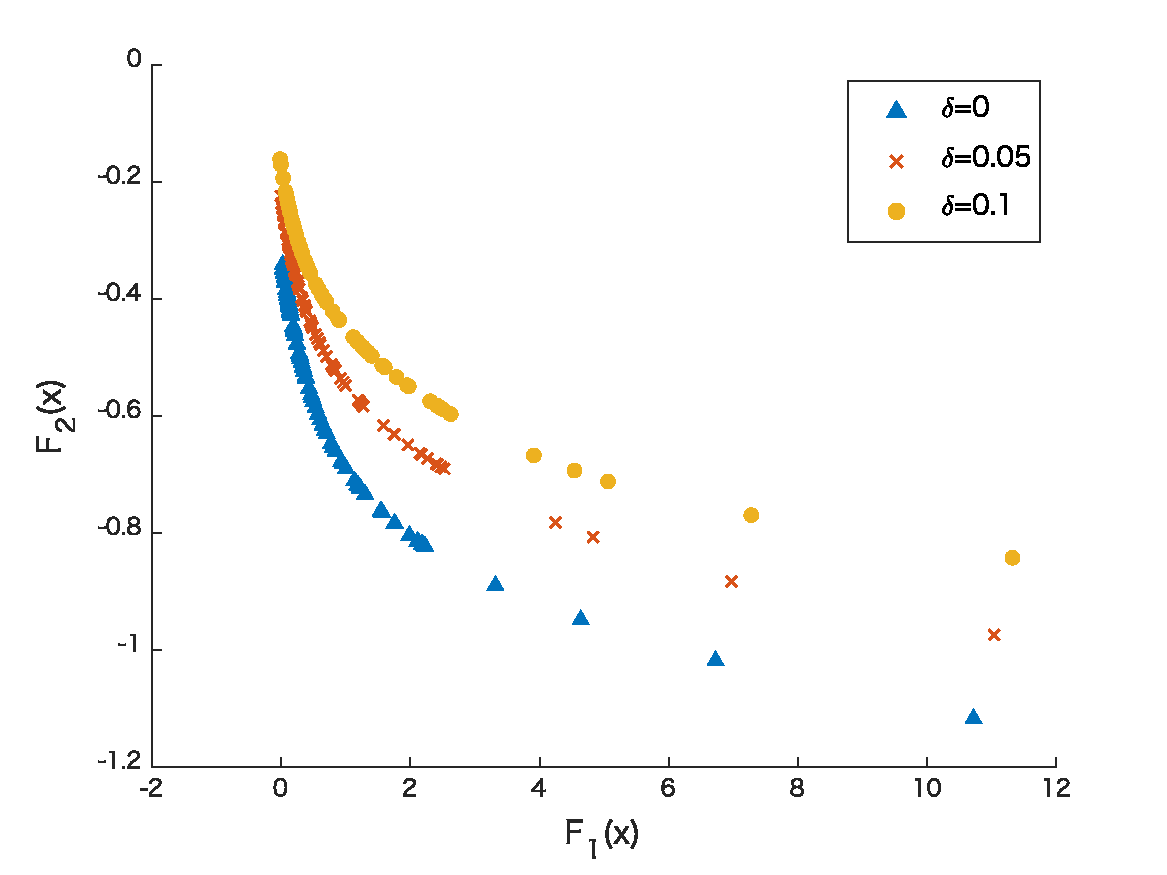
\includegraphics[clip, width = 7.0cm]{figs/linear_polyhedron_without_line_search}
\caption{Result for Experiment 1}
\label{fig:experiment1}
\end{figure}

\subsection*{Experiment 2}
In the second experiment, we solve the problem of \cref{sec:pgm:robust:SOCP}. We assume that $g_i(x) = \max_{u \in \mathcal{U}_i } u^\T x$, where $\mathcal{U}_i = \{u \in \setR^5 \mid \|u\| \leq \delta \},\, i = 1, 2$. We use the MATLAB solver \emph{SeDuMi}~\cite{Sturm1999} to solve \cref{eq:socp}. Figure \ref{fig:experiment2} is the result for this experiment. Once again, we obtained part of the Pareto frontier for the problems with and without uncertainties.
\begin{figure}[htbp]
\centering
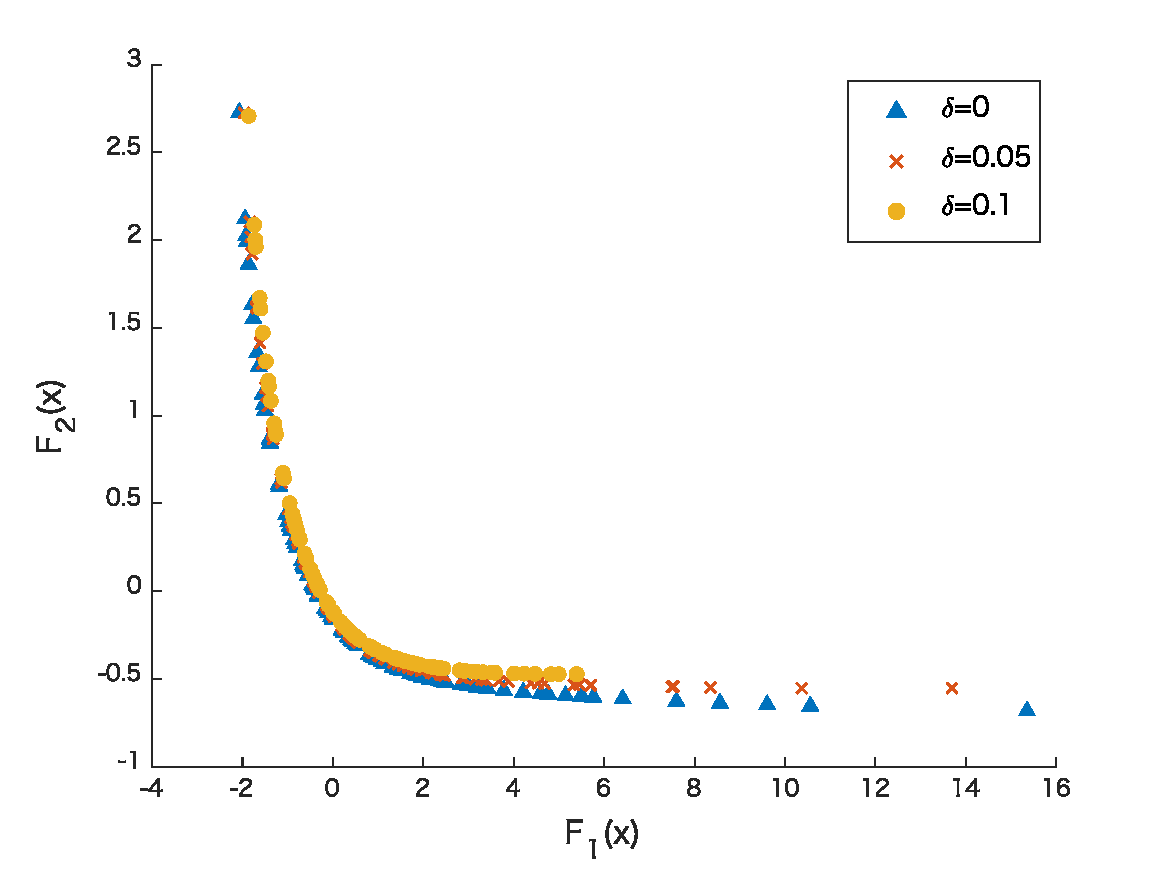
\includegraphics[clip, width = 7.0cm]{figs/linear_ellipsoid_without_line_search}
\caption{Result for Experiment 2}
\label{fig:experiment2}
\end{figure}
\begin{figure}[thbp]
\centering
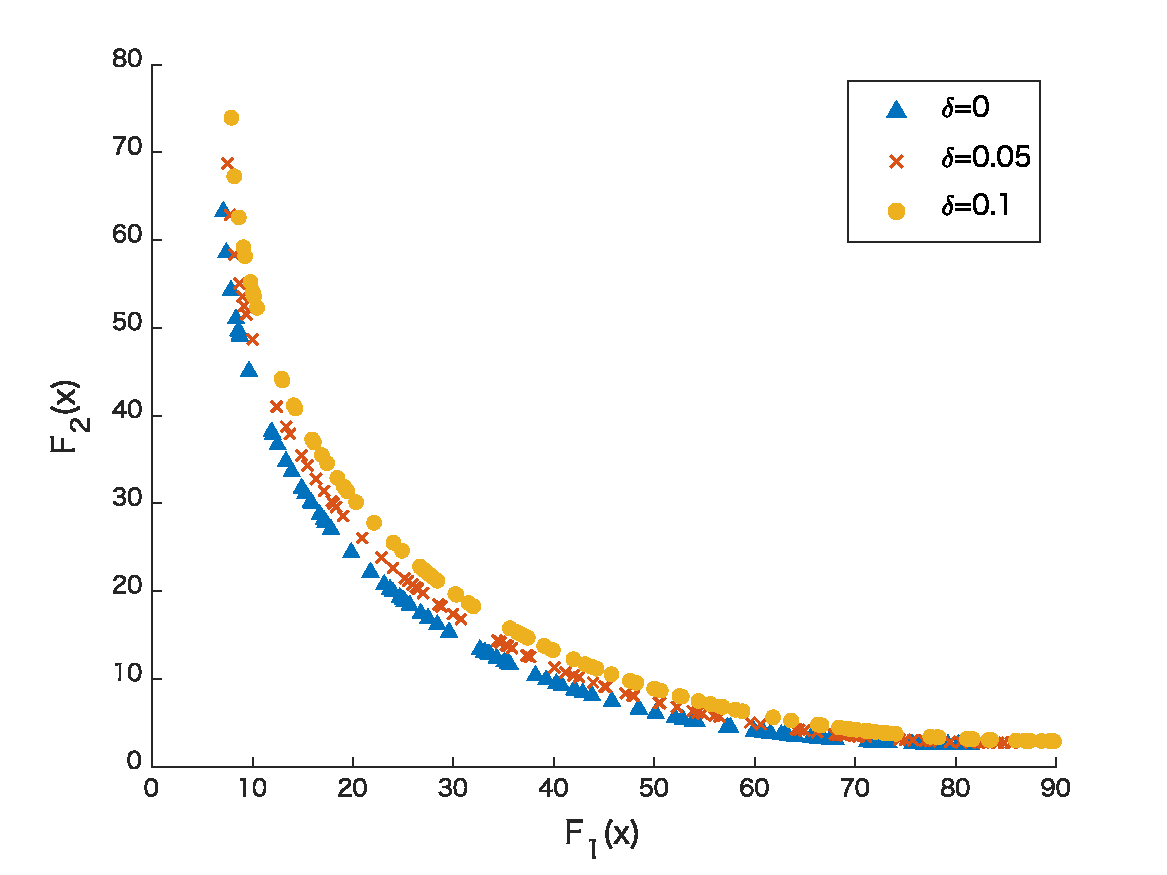
\includegraphics[clip, width = 7.0cm]{figs/quadratic_ellipsoid_without_line_search}
\caption{Result for Experiment 3}
\label{fig:experiment3}
\end{figure}
\subsection*{Experiment 3}
Now, in the last experiment, we solve the problem of \cref{sec:pgm:robust:SDP}. We assume that $g_i(x) = \max_{u \in \mathcal{U}_i } (u + x)^\T B B^\T (u + x)$, where $\mathcal{U}_i = \{u \in \setR^5\ | \  \|u\| \leq \delta \},\, i = 1, 2$. Here, once again, every component of $B \in \setR^{5 \times 5}$ is chosen randomly from the standard normal distribution and $\delta \geq 0$. We use the MATLAB solver \emph{fmincon} to solve \cref{eq:sdp_g_i} and \emph{SeDuMi} to solve \cref{eq:sdp}. As it can be seen in \cref{fig:experiment3}, we also obtained the Pareto frontier in this case.
\end{document}
